\RequirePackage[T1]{fontenc}
\documentclass[conference]{IEEEtran}
\usepackage{amsmath,amssymb,graphicx,booktabs,array,url}
\usepackage[hidelinks]{hyperref}
\pagestyle{plain}
\graphicspath{{figures/}}
\title{Independent Recurrent Models and Calibrated Hybrid Corrections for One-Hour PM2.5 Forecasting}
\author{\IEEEauthorblockA{\begin{tabular}{ccc}
\textbf{Samarth Khera} & \textbf{Pratham Malhotra} & \textbf{Adityaraj Pal}\\
2401010407 & 2401010343 & 2401010042\\[5pt]
\textbf{Tattva Rajput} & \textbf{Himanshu} & \\
2401010478 & 2401010188 &
\end{tabular}}\IEEEauthorblockA{CSAI Student Project 19 --- Phase 2: Deep Learning and Hybrid Forecasting}}
\begin{document}
\maketitle
\thispagestyle{plain}
\begin{abstract}
We extend a chronological Beijing PM2.5 forecasting study with independently trained LSTM and Bi-LSTM models, temporal-attention ablations, three-seed validation and a calibrated XGBoost correction head. Eight recurrent configurations are screened using 2013 data, followed by matched architecture/attention comparisons and hybrid selection. The final 2014 comparison uses the same 8,531 observed target hours for every method. Bi-LSTM achieves RMSE 20.799, LSTM 20.726, hybrid 20.919 and Ridge 21.063 micrograms per cubic meter. The validation-based preference is LSTM. Saved predictions, fold boundaries, source/data hashes and model artifacts support inspection and reproduction. The 2014 results remain exploratory because their Phase 1 counterparts were previously viewed.
\end{abstract}
\begin{IEEEkeywords}
PM2.5, recurrent forecasting, Bi-LSTM, attention, residual hybrid, chronological validation
\end{IEEEkeywords}

\section{Research Question and Scope}
We forecast the observed concentration $y_{t+1}$ from pollution, weather and calendar information available at origin $t$. The practical question is whether recurrent sequence models and a learned error correction add value beyond strong classical predictors. Our earlier Phase 1 experiment established persistence, seasonal naive, Ridge and XGBoost references. Phase 2 adds an independently fitted recurrent benchmark, validation-based model selection, matched attention and directionality comparisons, seed stability, a calibrated residual hybrid, and a local demonstration.

This is a historical Beijing study. The 2014 Phase 1 results had already been inspected before the current model development. Accordingly, every new 2014 comparison is explicitly exploratory. Chronological label boundaries prevent future observations from entering a fit, but do not turn an already-viewed year into a new blind test. We make no claim of statistical significance, present-day accuracy or transfer to another city.

A valid negative finding is part of the work: the complexity of a neural or hybrid model is not evidence of improved forecasting. We retain unsuccessful candidates, compare identical target hours and report peak errors separately. The final model preference is based on validation, not on whichever method has the most attractive 2014 number.

\section{Related Methods}
LSTM provides a gated recurrent representation for sequence inputs~\cite{pytorch}. We compare a forward LSTM with a bidirectional LSTM, where both directions operate entirely inside an already-observed input window. Temporal attention forms a learned weighted sum of these hidden states. Additive attention is motivated by the alignment formulation of Bahdanau et al.~\cite{attention}; their translation results are not used as comparable air-quality evidence.

For the hybrid, XGBoost learns a regularized nonlinear correction~\cite{xgboost}. Our contribution is the application and inspection of a chronological calibration protocol, rather than a claim to invent either recurrent networks or boosting. Scikit-learn's guidance on splitting and preprocessing~\cite{sklearn} motivates keeping learned transformations within their training boundary. Scores from different horizons or random-split studies are not directly compared with this experiment.

\section{Data and Forecast Information}
The UCI Beijing archive~\cite{uci} contains 43,824 hourly records from 2010 through 2014. Concentrations were measured at the US Embassy in Beijing; weather came from Beijing Capital International Airport. There are 2,067 missing concentrations (4.72\%), with no absent hourly timestamps in the supplied file. The loader verifies schema, dates, uniqueness, finite numeric values and the provenance checksum. It keeps missing observations in their hourly slots, excludes the row identifier and retains valid pollution peaks.

The existing feature construction is preserved: PM2.5 lags at offsets 0, 1, 2, 3, 6, 12, 24, 48, 72 and 168 hours; trailing means, population standard deviations and observation fractions; cyclic target-hour, weekday and month encodings; a weekend flag; weather at offsets 0, 1 and 24 hours; wind direction; and missingness indicators. The 70 original features become numeric and fold-encoded categorical inputs. Lag zero is observed at the forecast origin, not at the future target.

Times use the Beijing local clock. Forecast-time publication delays cannot be verified from this archive, so observed readings are assumed available at issuance. Target-hour measured weather is excluded. Missing labels are never filled for scoring. Learned imputation, category levels, input scaling and target scaling use only the actual training windows.

\section{Recurrent Forecasting Method}
For a sequence length $L$, the network receives
\begin{equation}
X_t=[x_{t-L+1},\ldots,x_t].
\end{equation}
The candidate lengths are 24 and 48 hours. A recurrent layer has 32 or 64 hidden units per direction, followed by a dense head with ReLU and dropout. Standardization and category encoding retain a frozen feature order at inference. Unknown future categories map to an all-zero known-category encoding, and missing numeric values use training medians.

With attention enabled, the hidden sequence $h_1,\ldots,h_L$ is summarized by
\begin{align}
e_i &= v^\top\tanh(Wh_i+b),\\
\alpha_i &= \frac{\exp(e_i)}{\sum_j\exp(e_j)},\qquad
c = \sum_i \alpha_i h_i.
\end{align}
Without attention, LSTM uses its final hidden state. Bi-LSTM concatenates the final forward and backward hidden states, so both directions summarize the complete observed window. Taking only the last row of bidirectional outputs would leave the backward component with only the most recent input; the audit corrected this before performing the ablation.

Two target formulations are screened. A level model predicts concentration directly; a delta model predicts a correction to current concentration. Let $b_t=0$ for level targets and $b_t=y_t$ for delta targets. If current pollution is missing, its training-median feature fill supplies this offset. The standardized target is
\begin{equation}
z_t=\frac{y_{t+1}-b_t-\mu_{\rm train}}{\sigma_{\rm train}},
\end{equation}
and the concentration forecast is
\begin{equation}
\hat y_{t+1}=\max\{0,b_t+\mu_{\rm train}+\sigma_{\rm train}g_\theta(X_t)\}.
\end{equation}
The network minimizes Huber loss with delta 1 in standardized units, using AdamW, learning rate 0.001, weight decay $10^{-4}$ and gradient-norm clipping at 1. Batch size is 128, dropout is 0.1, and candidates train for six or ten fixed epochs. There is no early stopping on 2014. Optimizing Huber loss is not equivalent to directly optimizing RMSE; this tradeoff matters when interpreting peak errors.

\section{Chronological Hybrid Calibration}
The standalone neural models now use every eligible row in the outer training window. This fixes the earlier benchmark's restriction to the hybrid's reduced base-training portion. The hybrid remains a separate estimator: reserve the last 10\% or 20\% of eligible training origins as a calibration block $C$, and fit the recurrent base on the earlier block $A$.

The latest base-training target must be observable by the first calibration origin. After base fitting, freeze its parameters and preprocessing. Compute calibration residuals
\begin{equation}
r_t=y_{t+1}-\hat y^{\rm base}_{t+1},\quad t\in C,
\end{equation}
and fit a tabular XGBoost model to $(x_t,r_t)$. The final forecast is
\begin{equation}
\hat y^{\rm hybrid}_{t+1}=\max\{0,\hat y^{\rm base}_{t+1}+\lambda\hat r_t\}.
\end{equation}
The correction weight $\lambda$ is selected from 0, 0.25, 0.5 and 1. The zero-weight control permits validation to reject the correction. Two tree configurations vary depth, estimator count, minimum child weight, learning rate and L2 regularization. No correction head trains on in-sample base residuals. The base is not refitted on the calibration labels afterward, including in the deployment model.

Every calibration target is available by the first evaluation origin. Fold audits retain base/calibration cutoffs, training rows, preprocessing boundaries, losses and random seeds. The hybrid's withheld calibration fraction is a methodological cost: it has less data for fitting its recurrent base than the independent standalone model. Any difference between those two estimators includes this training-data difference.

\section{Selection, Ablations and Evaluation}
The initial training period is 2010--2012. Four expanding quarterly 2013 folds supply validation; each model is fitted once at the quarter boundary using only already-available labels, while observed covariates update hourly. Four 2014 quarterly folds follow the same rule after selection. All methods use 8,563 common 2013 hours and 8,531 common 2014 hours. Common-hour scoring requires an observed target and both naive forecasts, avoiding model-specific removal of difficult hours.

The search is staged and recorded before evaluation. First, eight independent Bi-LSTM settings are screened at seed 42. This covers sequence length, width, duration, attention and target formulation. Next, the winning template supplies four matched variants: LSTM/Bi-LSTM crossed with attention on/off, each at seeds 42, 137 and 2026. The two architectures use the same per-direction hidden width; their parameter counts are consequently not identical. This is a controlled configuration comparison, not a parameter-budget-matched architecture claim.

For each architecture, attention is chosen using mean pooled validation RMSE across the three seeds. The selected Bi-LSTM configuration then supplies the hybrid base. Calibration fraction, residual-head settings and correction weight are selected by the same mean validation criterion. The search is deliberately finite and conditional on the first-stage template; it does not exhaust every combination or constitute nested cross-validation.

The model preference is compared with the classical validation references. The complete selection, including a hash of its evidence, is written before computing new 2014 scores. Seed 42 is fixed in advance for the historical comparison and saved deployment models; it is never chosen because of a favorable 2014 result. Seed standard deviations describe validation variability, not confidence intervals or significance tests.

For reproducibility, the neural seed controls initialization and shuffled minibatch order. XGBoost's residual head retains the Phase 1 random state of 42 while the neural seeds vary, so the reported hybrid seed variability does not measure every possible source of training randomness.

\begin{figure}[t]
\centering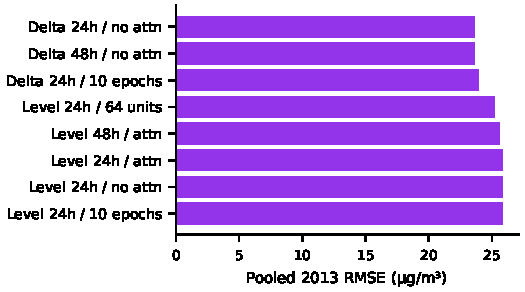
\includegraphics[width=\columnwidth]{article_validation_search.pdf}
\caption{All eight screened independent Bi-LSTM configurations, selected using 2013 only. Lower RMSE is better.}
\end{figure}
\begin{figure}[t]
\centering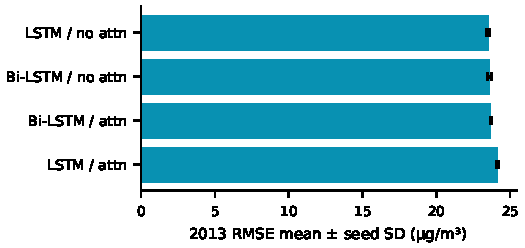
\includegraphics[width=\columnwidth]{article_attention_ablation.pdf}
\caption{Matched architecture/attention comparisons. Error bars are the standard deviation across three predefined validation seeds, not confidence intervals.}
\end{figure}

\section{Measured Findings}
The screening winner is \texttt{delta\_24h\_no\_attention}. The selected independent Bi-LSTM uses 24 input hours, 32 hidden units per direction, 6 epochs, disabled attention and a delta target. The selected hybrid reserves 20\% of eligible origins for calibration and uses correction weight 0.5. Its head configuration is recorded in the selection JSON. The selected Bi-LSTM and LSTM contain 29,505 and 14,241 trainable parameters, respectively. The model preferred by mean validation RMSE is LSTM.
\begin{table}[t]\centering
\caption{2014 exploratory comparison on identical observed target hours. Errors are in $\mu$g/m$^3$.}
\begin{tabular}{lrrr}\toprule
Model & MAE & RMSE & $R^2$\\\midrule
LSTM & 11.299 & 20.726 & 0.9506 \\
Bi-LSTM & 11.457 & 20.799 & 0.9503 \\
Bi-LSTM + XGBoost & 11.483 & 20.919 & 0.9497 \\
Ridge & 11.825 & 21.063 & 0.9490 \\
XGBoost & 11.833 & 21.088 & 0.9489 \\
Persistence & 11.926 & 22.033 & 0.9442 \\
Daily seasonal naive & 67.296 & 98.754 & -0.1205 \\
\bottomrule\end{tabular}\end{table}
The lowest observed pooled 2014 RMSE is 20.726 for LSTM. The independent Bi-LSTM RMSE is 20.799, compared with 22.033 for persistence and 21.063 for Ridge. The selected hybrid RMSE is 20.919. These are measured historical rankings, not evidence of statistical significance. The first corrected baseline used a shared reduced-training base, whereas this research run both changes model selection and trains standalone networks independently; differences between runs cannot be attributed to one factor alone.

\begin{table}[t]\centering
\caption{Selected-model validation stability. Mean and sample standard deviation across the three predefined seeds.}
\begin{tabular}{lrr}\toprule
Model & RMSE mean & RMSE SD\\\midrule
LSTM & 23.502 & 0.131 \\
Bi-LSTM & 23.613 & 0.132 \\
Bi-LSTM + XGBoost & 23.614 & 0.073 \\
\bottomrule\end{tabular}\end{table}
The seed table reports the variation of pooled 2013 errors for the selected configurations. Every seed uses the same target hours and chronological folds. A small seed standard deviation does not eliminate selection bias from repeatedly using one validation year. The 2014 table is a single predeclared seed, rather than a seed chosen after looking at final errors.

\begin{figure}[t]
\centering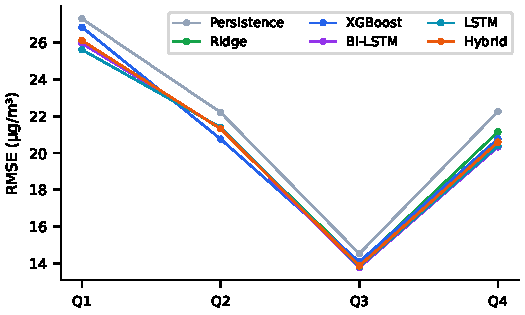
\includegraphics[width=\columnwidth]{article_quarterly_rmse.pdf}
\caption{Quarterly RMSE changes with season and pollution regime. Daily seasonal naive is omitted from this plot for scale and retained in the score table.}
\end{figure}

\subsection{Peak-Error Investigation}
A high-pollution threshold of 218 $\mu$g/m$^3$ is fixed from the initial training period's 90th percentile. The 2014 common target set contains 865 hours at or above this threshold and 7,666 below it. Each model uses the same observations within a regime.
The independent Bi-LSTM has high-pollution RMSE 37.902, LSTM 37.132, hybrid 38.587, Ridge 38.522 and persistence 38.557. Below the threshold, Bi-LSTM and hybrid RMSE are 17.870 and 17.860. The corresponding peak biases are -9.542 and -11.936; negative bias indicates underprediction. This stratification describes where errors occur. It does not establish a causal reason for a model failure. A correction that helps ordinary conditions can still degrade the pollution tail. The selected correction weight and regularization are chosen from validation, with no revision motivated by these 2014 regime scores. Isolating the correction on the same frozen base, pooled RMSE changes from 20.917 to 20.919; below-threshold RMSE changes from 18.018 to 17.860, while peak RMSE changes from 37.921 to 38.587. This isolates the contribution of the correction from differences in standalone training history.

\begin{figure}[t]
\centering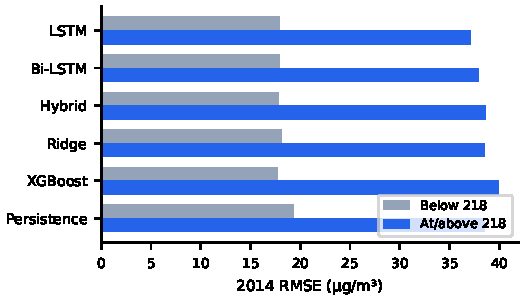
\includegraphics[width=\columnwidth]{article_pollution_regimes.pdf}
\caption{Low/peak regime errors use a threshold estimated from 2010--2012 only. Seasonal naive is omitted for scale. Overall improvement need not extend to pollution peaks.}
\end{figure}
\begin{figure}[t]
\centering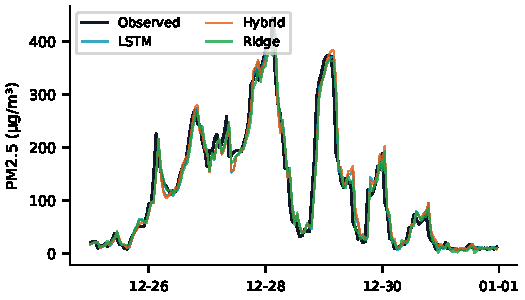
\includegraphics[width=\columnwidth]{article_forecast_last_week.pdf}
\caption{The last seven days of 2014, chosen by time rather than forecast success. Unscored target hours remain gaps.}
\end{figure}

\begin{figure}[t]
\centering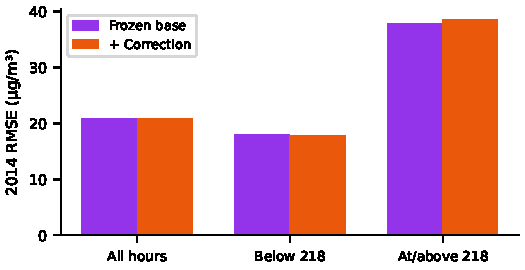
\includegraphics[width=\columnwidth]{article_correction_effect.pdf}
\caption{Correction effect isolated against the same frozen base, with unchanged target hours and fit. The reduced-training base differs from the independent Bi-LSTM benchmark.}
\end{figure}

\section{Audit, Verification and Deployment}
The first audit found full-dataset scaling, prediction-batch imputation, an unsafe training-mask fallback, omitted categorical wind inputs, in-sample residual training and suppressed correction errors. The corrected implementation learns transformations only from actual training windows, validates masks and hourly alignment, preserves wind categories, uses chronological calibration and propagates inference failures. A second audit corrected bidirectional state extraction without attention and separated the independent neural benchmark from the hybrid base.

A verified local CPU policy initializes numerical thread defaults before library imports. Optional neural exports load lazily. This avoids the reproduced macOS failure while deserializing mixed recurrent/XGBoost models. The CLI shares feature construction and sequence prediction with the dashboard; it no longer submits a single row to a sequence model.

The dashboard loads only a completed real-data run with matching model hashes. Classical models require 169 raw hourly slots; sequence models require $168+L$ slots so that every feature in the last $L$ input rows has its historical context. Manual inputs and uploaded histories produce matching CLI/dashboard forecasts. The local interface includes all available model scores, quarterly comparisons and export. Its hosted classical deployment is separate and does not package PyTorch.

The automated suite verifies future-feature/label invariance, frozen preprocessing, mask and hourly boundaries, delta reconstruction, bidirectional terminal states, calibration gaps, source/model hashes, selection-before-comparison, seed summaries, independent training counts and CLI prediction. Browser checks exercise model selection, performance tables, manual input, CSV upload/export, mobile layout and JavaScript errors. The submission retains the exact verification evidence alongside results.

\section{Reproducibility and Limitations}
The completed experiment records the source hash, input checksum, versions, all settings, selection evidence, seed scores, candidate predictions, fold audits and saved model hashes. An incomplete run may resume only when source, configuration and data agree. Checkpoints avoid repeating unchanged fits; completed runs are not overwritten. The original Phase 1 and first corrected Phase 2 outputs are preserved separately.

The submission includes this editable IEEE-format source and compiled PDF, editable presentation, matching slide PDF, presenter guide, training notebook, compact result tables, vector/raster figures and a runnable package with model weights and the attributed public dataset. The notebook loads the measured outputs by default and exposes an explicit switch to rerun the full experiment.

Scientific limitations remain. Model selection repeatedly uses the same 2013 year, so its scores are validation evidence rather than unbiased generalization estimates. A finite search and three seeds cannot establish universal architectural superiority. Prediction errors are temporally dependent; seed variation is not a calibrated estimate of uncertainty in future observations. The two sensor locations differ, weather publication delays are assumed, and the historical archive is specific to one city and period. We produce neither official AQI categories nor calibrated prediction intervals. A later untouched period or new dataset is needed for a new blind accuracy claim.

\section{Conclusion}
Phase 2 delivers independent recurrent benchmarks, validation selection, attention and directionality ablations, seed stability, chronological residual calibration and runnable saved models. Mean 2013 validation RMSE prefers LSTM; the lowest observed 2014 pooled RMSE is 20.726 for LSTM. The result is conditional on this archive, feature set and finite search. The scientific outcome is the measured comparison, including unsuccessful candidates and peak behavior, rather than an assumption that added complexity wins. A fresh untouched evaluation and broader data are required before making new generalization claims.

\begin{thebibliography}{9}
\bibitem{uci} S. Chen, ``Beijing PM2.5,'' UCI Machine Learning Repository, 2015. DOI: 10.24432/C5JS49. Dataset licensed CC BY 4.0.
\bibitem{pytorch} PyTorch contributors, ``LSTM,'' PyTorch 2.15 documentation. \url{https://docs.pytorch.org/docs/2.15/generated/torch.nn.LSTM.html}.
\bibitem{attention} D. Bahdanau, K. Cho and Y. Bengio, ``Neural Machine Translation by Jointly Learning to Align and Translate,'' ICLR, 2015. arXiv:1409.0473.
\bibitem{xgboost} T. Chen and C. Guestrin, ``XGBoost: A Scalable Tree Boosting System,'' KDD, 2016. arXiv:1603.02754.
\bibitem{sklearn} Scikit-learn contributors, ``Common pitfalls and recommended practices'' and ``Cross-validation.'' \url{https://scikit-learn.org/stable/common_pitfalls.html}.
\end{thebibliography}
\end{document}
